\documentclass[a4paper,twoside,12pt]{mgr}
\makeatletter
\def\@cite#1#2{{#1\if@tempswa , #2\fi}}
\makeatother
\usepackage{fancyhdr}
\pagestyle{fancy}
\usepackage{cite}
\usepackage{polski}
\usepackage[utf8]{inputenc}
\usepackage{float}
\restylefloat{figure}
\usepackage{listingsutf8}
\usepackage{color}
\usepackage{hyperref}
\usepackage{textcomp}
\definecolor{listinggray}{gray}{0.9}
\definecolor{lbcolor}{rgb}{0.9,0.9,0.9}

\lstset{
    inputencoding=utf8,
	backgroundcolor=\color{lbcolor},
	tabsize=4,
	rulecolor=,
	language=java,
        basicstyle=\scriptsize,
        upquote=true,
        aboveskip={1.5\baselineskip},
        columns=fixed,
        showstringspaces=false,
        extendedchars=true,
        breaklines=true,
        prebreak = \raisebox{0ex}[0ex][0ex]{\ensuremath{\hookleftarrow}},
        frame=single,
        showtabs=false,
        showspaces=false,
        showstringspaces=false,
        identifierstyle=\ttfamily,
        keywordstyle=\color[rgb]{0,0,1},
        commentstyle=\color[rgb]{0.133,0.545,0.133},
        stringstyle=\color[rgb]{0.627,0.126,0.941},
}
\usepackage{graphicx}
\fancyhf{}
\fancyhead[LE,LO]{\leftmark}
\fancyfoot[CE,CO]{- \thepage\ -}
%\linespread{1.3}
\fancypagestyle{plain}{
\fancyhead[LE,LO]{\leftmark}
\fancyfoot[CE,CO]{- \thepage\ -} 
}
\raggedbottom


%**************************************************************************
% Dane do strony tytułowej
%

% Autor
\autor{Piotr Zyszczak,Artur Śnioszek,Damian Łukasik}

% Rodzaj pracy - wpisać LICENCJACKA, INŻYNIERSKA lub MAGISTERSKA
\rodzajPracy{}

% Tytuł pracy magisterskiej/inżynierskiej
\tytul{Prognoza pogody}

% Rok
\rok{2016}

% Kierunek
\kierunek{Informatyka}

% Studia stacjonarne lub niestacjonarne (wpisać jakie)
\studia{stacjonarne}

% Poziom studiów wpisać I lub II
\poziomStudiow{II}


% Numer albumu
\numerAlbumu{113066,113055,112993}

%
%**************************************************************************


% Styl dla wtrąceń anglojęzycznych
\newcommand{\eng}[1]{(\emph{#1})}

\begin{document}

\stronaTytulowa

\tableofcontents
\chapter{Cel i zakres projektu}
Zaimplementować program zawierający technologie takie jak:
\begin{itemize}
\item System okienkowy
\item Grafika rastrowa oparta o GDI, Directx lub OpenGL
\item Wielowątkowość
\item Połączenie do bazy danych SQL
\item Połączenie sieciowe i obsługa sieci na poziomie gniazd z przejściem układu I/O na system wiadomości  windows(R) lub nowy watek z obsługą komunikacji sieciowej w technologii z obsługą gniazd bez przejścia z układu I/O na wiadomości systemu windows(R) (winsock.dll)  
\end{itemize}
Zdecydowano się więc na serwis pogodowy, który będzie pobierał dane z iternetu dzięki zapytaniom http.Połączenie z bazą bedzie tylko demonstracją technologii.


\chapter{Wykorzystane technologie}
Komendy Sekcji krytycznej:

CRITICALSECTION gSection;-inicjalizacja zmiannej

InitializeCriticalSection( \& g\_Section ); inicjalizacja sekcji

EnterCriticalSection( \& g\_Section ); 
	 	StatusWatek1=7;		-sekcja krytyczna ciało za zmiennymi których może kożystać 1 wątek
LeaveCriticalSection(\& g\_Section );

DeleteCriticalSection(\& g\_Section);-kasowanie sekcji krytycznej ogólnie zalończenie jej

Komendy do połączenia http:

WSAStartup(MAKEWORD(2,2), \&wsaData)-inicjalizacja użycia winsocka 

Makeword - wybiera wersję biblioteki. W tym przypadku 2.2.

\&wsaData - wskaźnik do struktury zawierającej informacje dotyczące implementacji Socketa

 gethostbyname("api.wunderground.com");-odbiera informacje odnoszące się do host z bazy hosta
 
 SOCKADDR\_IN SockAddr;
 
    SockAddr.sin\_port=htons(80); - wybieramy port 80
    
    SockAddr.sin\_family=AF\_INET; -korzystamy z wersji IPv4
    
    SockAddr.sin\_addr.s\_addr = *((unsigned long*)host->h\_addr);-przechowuje informacje o sockecie port na przykład
    
    connect(Socket,(SOCKADDR*)(\&SockAddr),sizeof(SockAddr))-ustawia połączenie dla danego socketa
    
    SOCKADDR*(\&SockAddr) - wskaźnik do struktury zawierającej informacje o adresie IP
    
    sizeof(SockAddr) - rozmiar wskaźnika
    
    send(Socket , mess , strlen(mess) , 0) -wysyła dane dla wyspecyfikowanego socketa. Mess - zapytanie do strony, strlen(mess) - długość zapytania
    
    recv(Socket,buffer,2000,0))-odbiera dane z połączonego socketa. Buffer - bufor na odbierane dane, 2000 - rozmiar bufora
    
    closesocket(Socket); - zamkanie Socketa
    
        WSACleanup();-funkcje zamykają socket i bibliotekę
        
  Komendy do bazy danych:
 
 SQLAllocHandle(SQL\_HANDLE\_ENV, SQL\_NULL\_HANDLE, \&sqlenvhandle)-alokuje środowisko , połączenie , stan, deskryptor. SQL\_HANDLE\_ENV - uchwyt do środowiska. SQL\_NULL\_HANDLE - uchwyt nadrzędny, w tym przypadku NULL. \&sqlenvhandle - wskaźnik do bufora, który zwraca uchwyt do zaalokowanej pamięci
 
   SQLRETURN SQLSetEnvAttr(
     SQLHENV      EnvironmentHandle, -uchwyt do środowiska
     SQLINTEGER   Attribute, - atrybut, którego wartość ma być zmieniona
     SQLPOINTER   ValuePtr, - wskaźnik do bufora z wartością dla atrybutu
     SQLINTEGER   StringLength);-ustawia atrybuty które regulują aspekty środowiska
     
    SQLRETURN SQLDriverConnect(
     SQLHDBC         ConnectionHandle, - uchwyt do połączenia
     SQLHWND         WindowHandle, - uchwyt do okna
     SQLCHAR *       InConnectionString, - odnośnik do sterownika w systemie
     SQLSMALLINT     StringLength1, -długość odnośnika do sterownika
     SQLCHAR *       OutConnectionString, - wskaźnik do bufora zawierającego nazwę sterownika
     SQLSMALLINT     BufferLength, - wielkość bufora w znakach
     SQLSMALLINT *   StringLength2Ptr, -wskaźnik do bufora zwracającego wielkość bufora w znakach
     SQLUSMALLINT    DriverCompletion);-łączy z sterownikiem do bazy danych
     
     SQLRETURN SQLExecDirect(
     SQLHSTMT     StatementHandle, - uchwyt do zapytania
     SQLCHAR *    StatementText, - zapytanie
     SQLINTEGER   TextLength);- długość zapytania
     odpala zapytania do bazy danych 
     
     SQLRETURN SQLFreeHandle(
     SQLSMALLINT   HandleType, - typ uchwytu
     SQLHANDLE     Handle);-uchwyt, który ma być zwolniony
     zwalnia zasoby połączone z środowiskiem itp.
     
     SQLRETURN SQLDisconnect(
     SQLHDBC     ConnectionHandle);-uchwyt do połączenia
     -zamyka połączenie powiązane z konkretnym handlerem
     
     Zmienne:
     
     WNDCLASSEX wc1;
	WNDCLASSEX wc2; struktura przechowujące informacje o oknie
	
	HWND hwnd;
	HWND hwnd2;
	HWND hwnd3; -uchwyty do okien
	
	HANDLE Handle\_Of\_Thread\_1 = 0; - uchwyt do wątku
	
	HWND hText,hText2;
	
	CRITICALSECTION g\_Section; 
	int StatusWatek1=-1;   -sekcja krytyczna 1 i jej status

		
		
		
	char buffer1[1024];
	char buffer\_w1[100000]; // dane z watku1 
	char dest\_buf\_w2[500]; // dane z watku2
	SQLCHAR message\_w2[500]; // komunikat bledu w2
     
     
  
 
\chapter{Implementacja}
W tym rozdziale opiszę po kolei funkcje i opowiem jak realizują założenia. Opis nalezy zacząć od głównej funkcji programu która wygląda naztępująco:
		
\begin{figure}[H]
\centering
\begin{lstlisting}[frame=single]		
int WINAPI WinMain(HINSTANCE hInstance, HINSTANCE hPrevInstance, LPSTR lpCmdLine, int nCmdShow) {
	InitializeCriticalSection( & g_Section );
	InitializeCriticalSection( & g_Section1 );
	WNDCLASSEX wc; /* A properties struct of our window */
	MSG msg; /* A temporary location for all messages */

	/* zero out the struct and set the stuff we want to modify */
	memset(&wc,0,sizeof(wc));
	wc.cbSize		 = sizeof(WNDCLASSEX);
	wc.lpfnWndProc	 = WndProc; /* This is where we will send messages to */
	wc.hInstance	 = hInstance;
	wc.hCursor		 = LoadCursor(NULL, IDC_ARROW);
	
	/* White, COLOR_WINDOW is just a #define for a system color, try Ctrl+Clicking it */
	wc.hbrBackground = (HBRUSH)(COLOR_WINDOW+1);
	wc.lpszClassName = "WindowClass";
	wc.hIcon		 = LoadIcon(NULL, IDI_APPLICATION); /* Load a standard icon */
	wc.hIconSm		 = LoadIcon(NULL, IDI_APPLICATION); /* use the name "A" to use the project icon */
	
/* zero out the struct and set the stuff we want to modify */
					memset(&wc1,0,sizeof(wc1));
					wc1.cbSize		 = sizeof(WNDCLASSEX);
					wc1.lpfnWndProc	 = WndProc1; /* This is where we will send messages to */
					wc1.hInstance	 = hInstance;
					wc1.hCursor		 = LoadCursor(NULL, IDC_ARROW);
	
					/* White, COLOR_WINDOW is just a #define for a system color, try Ctrl+Clicking it */
					wc1.hbrBackground = (HBRUSH)(COLOR_WINDOW+1);
					
\end{lstlisting}
\caption{Główna funkcja.}%
\label{rys:etykieta}
\end{figure}	

\begin{figure}[H]
\centering
\begin{lstlisting}[frame=single]	
					wc1.lpszClassName = "WindowClass1";
					wc1.hIcon		 = LoadIcon(NULL, IDI_APPLICATION); /* Load a standard icon */
					wc1.hIconSm		 = LoadIcon(NULL, IDI_APPLICATION); /* use the name "A" to use the project icon */
					
					/* zero out the struct and set the stuff we want to modify */
					memset(&wc2,0,sizeof(wc2));
					wc2.cbSize		 = sizeof(WNDCLASSEX);
					wc2.lpfnWndProc	 = WndProc2; /* This is where we will send messages to */
					wc2.hInstance	 = hInstance;
					wc2.hCursor		 = LoadCursor(NULL, IDC_ARROW);
					/* White, COLOR_WINDOW is just a #define for a system color, try Ctrl+Clicking it */
					wc2.hbrBackground = (HBRUSH)(COLOR_WINDOW+1);
					wc2.lpszClassName = "WindowClass2";
					wc2.hIcon		 = LoadIcon(NULL, IDI_APPLICATION); /* Load a standard icon */
					wc2.hIconSm		 = LoadIcon(NULL, IDI_APPLICATION); /* use the name "A" to use the project icon */


	
	if(!RegisterClassEx(&wc)) {
		MessageBox(NULL, "Window Registration Failed!","Error!",MB_ICONEXCLAMATION|MB_OK);
		return 0;
	}
	
	if(!RegisterClassEx(&wc1)) {
		MessageBox(NULL, "Window Registration Failed!","Error!",MB_ICONEXCLAMATION|MB_OK);
		return 0;
	}
	
	if(!RegisterClassEx(&wc2)) {
		MessageBox(NULL, "Window Registration Failed!","Error!",MB_ICONEXCLAMATION|MB_OK);
		return 0;
	}
	
	
	\end{lstlisting}
\caption{Główna funkcja.}%
\label{rys:etykieta}
\end{figure}	

\begin{figure}[H]
\centering
\begin{lstlisting}[frame=single]	
hwnd = CreateWindowEx(WS_EX_CLIENTEDGE, - rozszerzone style okien
		"WindowClass", -nazwa klasy okna
		"Okno glowne", - nazwa wyswietlana na oknie
		WS_VISIBLE|WS_OVERLAPPEDWINDOW, -podstawowe style okien
		CW_USEDEFAULT, /* x */ wspolrzedna x
		CW_USEDEFAULT, /* y */ wspolrzedna y
		420, /* width */ szerokosc okna
		350, /* height */  wysokosc okna
		NULL, uchwyt do okna nadrzednego
		NULL, uchwyt do menu
		hInstance, -uchwyt do aplikacji
		NULL); wskaznik do struktury, przez ktora mozna przesylac dodatkowe informacje

	if(hwnd == NULL) {
		MessageBox(NULL, "Window Creation Failed!","Error!",MB_ICONEXCLAMATION|MB_OK);
		NULL - uchwyt do okna wlasciciela
		Windows Creation Failed! - tekst komunikatu
		Error - tekst wyswietlany na pasku okna
		MB_OK - przycisk
		return 0;
	}
	hwnd2 = CreateWindowEx(WS_EX_CLIENTEDGE,"WindowClass1","Prognoza",WS_VISIBLE|WS_OVERLAPPEDWINDOW,
		CW_USEDEFAULT, /* x */
		CW_USEDEFAULT, /* y */
		420, /* width */
		350, /* height */
		NULL,NULL,hInstance,NULL);

	if(hwnd2 == NULL) {
		MessageBox(NULL, "Window Creation Failed!","Error!",MB_ICONEXCLAMATION|MB_OK);
		return 0;
	}
	
	hwnd3 = CreateWindowEx(WS_EX_CLIENTEDGE,"WindowClass2","Autorzy",WS_VISIBLE|WS_OVERLAPPEDWINDOW,
		CW_USEDEFAULT, /* x */
		CW_USEDEFAULT, /* y */
		420, /* width */
		350, /* height */
		NULL,NULL,hInstance,NULL);

	if(hwnd3 == NULL) {
		MessageBox(NULL, "Window Creation Failed!","Error!",MB_ICONEXCLAMATION|MB_OK);
		return 0;
	}

	GenerateButtons(hwnd, hInstance); - hwnd - uchwyt do okna, hInstance - uchwyt do aplikacji
	GenerateButtonsWeather(hwnd2, hInstance);
	GenerateButtonsAuthors(hwnd3, hInstance);
	
	ShowWindow(hwnd2,SW_HIDE);
	hwnd2 - uchwyt do okna
	Zmienia stan okna. SW_HIDE - ukrywa dane okno i uaktywnia inne.
	ShowWindow(hwnd3,SW_HIDE);
\end{lstlisting}
\caption{Główna funkcja.}%
\label{rys:etykieta}
\end{figure}	

\begin{figure}[H]
\centering
\begin{lstlisting}[frame=single]	
	/*
		This is the heart of our program where all input is processed and 
		sent to WndProc. Note that GetMessage blocks code flow until it receives something, so
		this loop will not produce unreasonably high CPU usage
	*/
	while(GetMessage(&msg, NULL, 0, 0) > 0) { Pobiera wiadomosc msg. NULL - uchwyt do okna. Ostatnie 2 parametry to wartosc minimalna i 			maksymalna pobieranych wiadomosci. 
		TranslateMessage(&msg); Tlumaczenie wiadomosci na znaki.
		DispatchMessage(&msg); Przesylanie wiadomosci w odpowiednie miejsce.
		
	}
	DeleteCriticalSection(& g_Section); Usuwanie sekcji krytycznej.
	DeleteCriticalSection(& g_Section1);
	return msg.wParam;
}
\end{lstlisting}
\caption{Główna funkcja.}%
\label{rys:etykieta}
\end{figure}		

W funkcji głównej znajdziemy przede wszystkim informacje o liczbie okien, kolorze tła, rozmiarze, nagłówkach. Są tam też odniesienia do funkcji gdzie znajdują się reakcje na zdarzenia.

\begin{figure}[H]
\centering
\begin{lstlisting}[frame=single]	
LRESULT CALLBACK WndProc(HWND hwnd, UINT Message, WPARAM wParam, LPARAM lParam) {
	switch(Message) {
		/* Upon destruction, tell the main thread to stop */
		case WM_CLOSE: { przypadek zamkniecia glownego okna
			switch(MessageBox(NULL, "Chcesz zamknac?","Zamykanie?",MB_ICONQUESTION|MB_YESNO)){
						case IDYES:{
							PostQuitMessage(0);
							break;
						}
						case IDNO:{
							MessageBox(NULL, "Nie!","Ups",MB_ICONINFORMATION|MB_OK);
							break;
						}
			}
			break;
		}
		
		case WM_COMMAND: {
			switch(wParam) {
				case B_Option1: {
				
				ShowWindow(hwnd2,SW_SHOW);	
					
					break;
				}
				case B_Option2: {
					
				ShowWindow(hwnd3,SW_SHOW);	
				
					break;	
				}
				case B_Option3: {
					switch(MessageBox(NULL, "Chcesz zamknac?","Zamykanie?",MB_ICONQUESTION|MB_YESNO)){
						case IDYES:{
							PostQuitMessage(0);
							break;
						}
						case IDNO:{
							MessageBox(NULL, "Nie!","Odmowa",MB_ICONINFORMATION|MB_OK);
							break;
\end{lstlisting}
\caption{Główne menu.}%
\label{rys:etykieta}
\end{figure}	

\begin{figure}[H]
\centering
\begin{lstlisting}[frame=single]	
												}
					break;
					}
				}
				default: {
					break;
				}
			}
			break;
		}
		case WM_PAINT: {
			OnPaint(hwnd);
			break;
		}
		
		/* All other messages (a lot of them) are processed using default procedures */
		default:
			return DefWindowProc(hwnd, Message, wParam, lParam);
	}
	return 0;
}
\end{lstlisting}
\caption{Główne menu.}%
\label{rys:etykieta}
\end{figure}

Jak można zauważyć powyżej zdażenia są przechwytywane i rozpatrywane za pomocą funkcji switch. Funkcja ta rozpoznaje wcześniej zdefiniowaną nazwę przycisku i reaguje w sosób zdefiniowany przez programistę dla konkretnego przycisku. Można też dostrzec iż mechanizm okienkowy został zaimplementowany przy pomocy funkcji chowających i pokazujących okna gdyż nie było potrzeby ich tworzenia przy każdym naciśnięciu przycisku. Z tejże funkcji uruchamiana jest też funkcja rysująca przykłądową grafikę.

\begin{figure}[H]
\centering
\begin{lstlisting}[frame=single]	
LRESULT OnPaint(HWND hwnd){
	PAINTSTRUCT ps;
	HDC hdc; kontekst urzadzenia
	int l=0;
	//static int x,y;

	hdc = BeginPaint(hwnd, &ps);
	RECT rect;
	GetClientRect(hwnd, &rect); pobranie rozmiarow danego okna
	
	HBRUSH brush = CreateSolidBrush(RGB(0,0,255)); utworzenie pedzla o wybranym kolorze
	//FillRect(hdc, &rect, brush);
	SelectObject(hdc, brush); wybranie nowego obiektu do kontektstu urzadzenia
	
	
	//Rainy claud
	Ellipse(hdc ,200,150,250,200 );
	Ellipse(hdc ,230,150,280,200 );
	Ellipse(hdc ,260,150,310,200 );
	Ellipse(hdc ,290,150,340,200 );
	l+=10;//+l
	Ellipse(hdc ,200+l,150+l,250+l,200 +l);
	Ellipse(hdc ,230+l,150+l,280+l,200 +l);
	Ellipse(hdc ,260+l,150+l,310+l,200+l );
	Ellipse(hdc ,290+l,150+l,340+l,200+l );
	MoveToEx(hdc, rect.left + 210, rect.top + 220, NULL);
	LineTo(hdc, rect.left + 210, rect.top + 250);
	MoveToEx(hdc, rect.left + 230, rect.top + 220, NULL);
	LineTo(hdc, rect.left + 230, rect.top + 250);
	MoveToEx(hdc, rect.left + 250, rect.top + 220, NULL);
	LineTo(hdc, rect.left + 250, rect.top + 250);
	MoveToEx(hdc, rect.left + 270, rect.top + 220, NULL);
	LineTo(hdc, rect.left + 270, rect.top + 250);
	MoveToEx(hdc, rect.left + 290, rect.top + 220, NULL);
	LineTo(hdc, rect.left + 290, rect.top + 250);
	MoveToEx(hdc, rect.left + 310, rect.top + 220, NULL);
	LineTo(hdc, rect.left + 310, rect.top + 250);
	MoveToEx(hdc, rect.left + 330, rect.top + 220, NULL);
	LineTo(hdc, rect.left + 330, rect.top + 250);
	
	EndPaint(hwnd, &ps);
	DeleteObject(brush);
}
\end{lstlisting}
\caption{Funkcja graficzna.}%
\label{rys:etykieta}
\end{figure}

Funkcja ta przy pomocy komend graficznych rysuje chmurę za pomocą prostych kształtów (linii i kółek) co realizuje jeden z punktów.

\begin{figure}[H]
\centering
\begin{lstlisting}[frame=single]	
void GenerateButtons(HWND parent, HINSTANCE hInstance){
	CreateWindow(TEXT("STATIC"), TEXT("Witaj w programie Prognoza Pogody."),
                              WS_CHILD | WS_VISIBLE ,
                              10, 10, 350, 25,
                              parent, (HMENU)(502),
                              hInstance, NULL);
		
	CreateWindowEx(WS_EX_CLIENTEDGE,"Button","Wyszukaj Pogode",WS_VISIBLE|WS_CHILD|BS_PUSHBUTTON,
		50, /* x */
		50, /* y */
		130, /* width */
		30, /* height */
		parent,(HMENU)B_Option1,hInstance,NULL);
	
	CreateWindowEx(WS_EX_CLIENTEDGE,"Button","Autorzy",WS_VISIBLE|WS_CHILD|BS_PUSHBUTTON,
		50, /* x */
		90, /* y */
		70, /* width */
		30, /* height */
		parent,(HMENU)B_Option2,hInstance,NULL);
		
	CreateWindowEx(WS_EX_CLIENTEDGE,"Button","Koniec",WS_VISIBLE|WS_CHILD|BS_PUSHBUTTON,
		50, /* x */
		130, /* y */
		70, /* width */
		30, /* height */
		parent,(HMENU)B_Option3,hInstance,NULL);
}
\end{lstlisting}
\caption{Funkcja tworząca kontrolki do menu głównego.}%
\label{rys:etykieta}
\end{figure}
Przyciski powstały w osobnej funkcji by ułatwić znalezienie ich.
\begin{figure}[H]
\centering
\begin{lstlisting}[frame=single]	
LRESULT CALLBACK WndProc2(HWND hwnd, UINT Message, WPARAM wParam, LPARAM lParam) {
	switch(Message) {
		
		/* Upon destruction, tell the main thread to stop */
		case WM_CLOSE: {
			switch(MessageBox(NULL, "Chcesz zamknac?","Zamykanie?",MB_ICONQUESTION|MB_YESNO)){
						case IDYES:{
							ShowWindow(hwnd,SW_HIDE);
							break;
						}
						case IDNO:{
							MessageBox(NULL, "Nie!","Ups",MB_ICONINFORMATION|MB_OK);
							break;
						}
					}
			break;
		}
		
		case WM_COMMAND: {
			switch(wParam) {
				case Closing: {
					ShowWindow(hwnd,SW_HIDE);
					//MessageBox(NULL, "Nie!","Odmowa",MB_ICONINFORMATION|MB_OK);
					break;
				}
			}
			break;
		}
		
		/* All other messages (a lot of them) are processed using default procedures */
		default:
			return DefWindowProc(hwnd, Message, wParam, lParam);
	}
	return 0;
\end{lstlisting}
\caption{Spis autorów.}%
\label{rys:etykieta}
\end{figure}
Zdarzenia dla okna wypisującego autorów programu.
\begin{figure}[H]
\centering
\begin{lstlisting}[frame=single]	
void GenerateButtonsAuthors(HWND parent, HINSTANCE hInstance){
	
	//static HWND hwnd_ed_u;
	CreateWindow(TEXT("STATIC"), TEXT("Mamy nastepujacy sklad:"),
                              WS_CHILD | WS_VISIBLE ,
                              50, 10, 200, 25,
                              parent, (HMENU)(502),
                              hInstance, NULL);
							  	
	CreateWindow(TEXT("STATIC"), TEXT("inz. Piotr Zyszczak"),
                              WS_CHILD | WS_VISIBLE ,
                              50, 50, 200, 25,
                              parent, (HMENU)(502),
                              hInstance, NULL);
                              
    CreateWindow(TEXT("STATIC"), TEXT("inz Artur Snioszek"),
                              WS_CHILD | WS_VISIBLE ,
                              50, 90, 200, 25,
                              parent, (HMENU)(502),
                              hInstance, NULL);   
                              
	CreateWindow(TEXT("STATIC"), TEXT("inz Damian Lukasik"),
                              WS_CHILD | WS_VISIBLE ,
                              50, 130, 200, 25,
                              parent, (HMENU)(502),
                              hInstance, NULL);  
                              
	CreateWindowEx(WS_EX_CLIENTEDGE,"Button","Zamknij",WS_VISIBLE|WS_CHILD|BS_PUSHBUTTON,
		50, /* x */
		170, /* y */
		130, /* width */
		30, /* height */
		parent,(HMENU)Closing,hInstance,NULL);                      
}
\end{lstlisting}
\caption{Kontrolki do spisu autorów.}%
\label{rys:etykieta}
\end{figure}
Funkcja robi to samo co tworząca kontrolki dla menu.

\begin{figure}[H]
\centering
\begin{lstlisting}[frame=single]	
LRESULT CALLBACK WndProc1(HWND hwnd, UINT Message, WPARAM wParam, LPARAM lParam) {
	
	
	int Data_Of_Thread_1 = 1;
	int Data_Of_Thread_2 = 1;
	HANDLE Array_Of_Thread_Handles[3];
	switch(Message) {
		
		/* Upon destruction, tell the main thread to stop */
		case WM_CLOSE: {
			switch(MessageBox(NULL, "Chcesz zamknac?","Zamykanie?",MB_ICONQUESTION|MB_YESNO)){
						case IDYES:{
							ShowWindow(hwnd,SW_HIDE);
							break;
						}
						case IDNO:{
							MessageBox(NULL, "Nie!","Ups",MB_ICONINFORMATION|MB_OK);
							break;
						}
			}
			break;
		}
		
		case WM_COMMAND: {
			switch(wParam) {
				case Closing2: {
					ShowWindow(hwnd,SW_HIDE);
					break;
				}
				case Chconn: {
					//InitializeCriticalSection( & g_Section );
					HANDLE Handle_Of_Thread_1 = CreateThread( NULL, 0,FunkcjaConnectowa, &Data_Of_Thread_1, 0, NULL);
					//Array_Of_Thread_Handles[0] = Handle_Of_Thread_1;
					//WaitForSingleObject( Handle_Of_Thread_1, 500);
					DWORD rs = WaitForSingleObject( Handle_Of_Thread_1, 10000);
				
					
					if(rs == WAIT_OBJECT_0)
					{
						MessageBox(NULL,"Watek zakonczyl sie","Komunikat",MB_ICONINFORMATION|MB_OK);	 
					}
					
\end{lstlisting}
\caption{Zdarzenia okna prezentującego pogodę.}%
\label{rys:etykieta}
\end{figure}
\begin{figure}[H]
\centering
\begin{lstlisting}[frame=single]
					else if(rs == WAIT_TIMEOUT)
					{
						MessageBox(NULL,"Przekroczono czas","Komunikat",MB_ICONINFORMATION|MB_OK);	        		
					}else if(rs == WAIT_FAILED)
					{
						MessageBox(NULL,"Funkcja nie powiodla sie","Komunikat",MB_ICONINFORMATION|MB_OK);	        		
					}
					else if(rs == WAIT_ABANDONED)
					{
						MessageBox(NULL,"Blad","Komunikat",MB_ICONINFORMATION|MB_OK);	  
					}
					//MessageBox(NULL,buffer,"Watek pogodowy",MB_ICONINFORMATION|MB_OK);
				
					//DeleteCriticalSection(& g_Section);
					CloseHandle(Handle_Of_Thread_1);
						
					if (StatusWatek1==-1) {
						MessageBox(NULL,"Watek nie uruchomiony","Komunikat",MB_ICONINFORMATION|MB_OK);
					}
					else if (StatusWatek1==0) {
						MessageBox(NULL,"Zakonczono pobieranie","Komunikat",MB_ICONINFORMATION|MB_OK);
					}
					else if (StatusWatek1==1) {
						MessageBox(NULL,"Nadal pobieram dane","Komunikat",MB_ICONINFORMATION|MB_OK);
					}
					else if(StatusWatek1==2) {
						MessageBox(NULL,"Wysylam zapytanie","Komunikat",MB_ICONINFORMATION|MB_OK);
					}
					else if(StatusWatek1==3) {
						MessageBox(NULL,"Blad w funkcji connect","Komunikat",MB_ICONINFORMATION|MB_OK);
					}
					
\end{lstlisting}
\caption{Zdarzenia okna prezentującego pogodę.}%
\label{rys:etykieta}
\end{figure}
\begin{figure}[H]
\centering
\begin{lstlisting}[frame=single]
				else if(StatusWatek1==4) {
						MessageBox(NULL,"Blad inicjacji wsastartup","Komunikat",MB_ICONINFORMATION|MB_OK);
					}
					else if(StatusWatek1==7) {
						MessageBox(NULL,"Nie ma Internetu","Komunikat",MB_ICONINFORMATION|MB_OK);
					}
					MessageBox(NULL,buffer_w1,"Komunikat",MB_ICONINFORMATION|MB_OK);
					memset(buffer_w1, 0, sizeof buffer_w1);
					break;
				}
				case DBtest: {
					//InitializeCriticalSection( & g_Section1 );
					HANDLE Handle_Of_Thread_2 = CreateThread( NULL, 0,FunkcjaBazodanowa, &Data_Of_Thread_2, 0, NULL);
					if (WaitForSingleObject( Handle_Of_Thread_2,100000) !=WAIT_TIMEOUT){
					if(StatusWatek2==0){
						MessageBox(NULL, "Blad w watku!","Blad!",MB_ICONINFORMATION|MB_OK);
					}
					if(StatusWatek2==1){
						MessageBox(NULL, dest_buf_w2,"Wszystko ok!",MB_ICONINFORMATION|MB_OK);
					}
					if(StatusWatek2==2){
						MessageBox(NULL, message_w2,"Blad wdostepie do bazy!",MB_ICONINFORMATION|MB_OK);
					}
					}
        			else{
    					MessageBox(NULL,"Proces przekroczyl czas!","Wszystko ok",MB_ICONINFORMATION|MB_OK);
					}
					memset(dest_buf_w2, 0, sizeof dest_buf_w2);
					memset(message_w2, 0, sizeof message_w2);
					CloseHandle(Handle_Of_Thread_2);
					break;
				}
			}
			break;
		}
		
		/* All other messages (a lot of them) are processed using default procedures */
		default:
			return DefWindowProc(hwnd, Message, wParam, lParam);
	}
	return 0;
}
\end{lstlisting}
\caption{Zdarzenia okna prezentującego pogodę.}%
\label{rys:etykieta}
\end{figure}
W pewnym sensie nowością w tym oknie jest zastosowanie wątków do wywołania funkcji które będą ciałami tych wątków (funkcja createThread). Dodatkowo można wspomnieć o mechaniźmie zmiennych oznaczających różne fazy wątku np.Brak internetu spowoduje awaryjne wyjście z funkcji w wątku wywołanym z kalwisza zdefiniowanego jako Chconn. W obu pewne dane trzeba było przekazać do głównego wątku. By te nie kolidowały ze sobą użyto mechanizmu sesji krytycznej.

\begin{figure}[H]
\centering
\begin{lstlisting}[frame=single]
int FunkcjaConnectowa(){
	
	char buffer[100000];
	buffer[0] = 0;
	
	
	char *mess;
	
	WSADATA wsaData;
    if (WSAStartup(MAKEWORD(2,2), &wsaData) != 0) {
       // MessageBox(NULL, "dsa","WSA startup failed",MB_ICONINFORMATION|MB_OK);
        EnterCriticalSection( & g_Section );
	 	StatusWatek1=4;
	 	LeaveCriticalSection( & g_Section );
        system("pause");
        return 1;
    }
  
    SOCKET Socket=socket(AF_INET,SOCK_STREAM,IPPROTO_TCP);
    struct hostent *host;
    
    host = gethostbyname("api.wunderground.com");
    if(host != NULL){
    }
    else{
		EnterCriticalSection( & g_Section );
	 	StatusWatek1=7;
	 	LeaveCriticalSection( & g_Section );
	 	system("pause");
	 	return 1;}
	//WSACleanup();

    SOCKADDR_IN SockAddr;
    SockAddr.sin_port=htons(80);
    SockAddr.sin_family=AF_INET;
    SockAddr.sin_addr.s_addr = *((unsigned long*)host->h_addr);
 \end{lstlisting}
\caption{Funkcja pobierająca dane z internetu.}%
\label{rys:etykieta}
\end{figure}
\begin{figure}[H]
\centering
\begin{lstlisting}[frame=single]   
    if(connect(Socket,(SOCKADDR*)(&SockAddr),sizeof(SockAddr)) != 0){
        EnterCriticalSection( & g_Section );
	 	StatusWatek1=3;
	 	LeaveCriticalSection( & g_Section );
        system("pause");
        return 1;
    }
    
   	DWORD dlugosc = GetWindowTextLength( hText );
	LPSTR Bufor =( LPSTR ) GlobalAlloc( GPTR, dlugosc + 1 );
	GetWindowText( hText, Bufor, dlugosc + 1 );
	
	DWORD dlugosc2 = GetWindowTextLength( hText2 );
	LPSTR Bufor2 =( LPSTR ) GlobalAlloc( GPTR, dlugosc2 + 1 );
	GetWindowText( hText2, Bufor2, dlugosc2 + 1 );
	
	
	char* char1=(char*)Bufor;
	char* char2=(char*)Bufor2;
	char* char3= "GET /api/5df3f8dcf842e4e7/geolookup/conditions/forecast/q/";
	char* char4= "/";
	char* char5= ".json HTTP/1.1\r\nHost: api.wunderground.com\r\n\r\n";
	char dest_buf[100]; 
	wsprintf (dest_buf, "%s%s", char3, char1);
	wsprintf (dest_buf, "%s%s", dest_buf, char4);
	wsprintf (dest_buf, "%s%s", dest_buf, char2);
	wsprintf (dest_buf, "%s%s", dest_buf, char5);

 \end{lstlisting}
\caption{Funkcja pobierająca dane z internetu.}%
\label{rys:etykieta}
\end{figure}
\begin{figure}[H]
\centering
\begin{lstlisting}[frame=single] 	
	mess = dest_buf;
    if(send(Socket , mess , strlen(mess) , 0) < 0)
    {
        EnterCriticalSection( & g_Section );
	 	StatusWatek1=2;
	 	LeaveCriticalSection( & g_Section );
    }
	
    int nDataLength;
    
   
    while ((nDataLength = recv(Socket,buffer,2000,0)) > 0){        
        
       // MessageBox(NULL, buffer, "Connecting",MB_ICONINFORMATION|MB_OK);
        EnterCriticalSection( & g_Section );
        wsprintf (buffer_w1, "%s%s", buffer_w1, buffer);
	 	StatusWatek1=1;
	 	LeaveCriticalSection( & g_Section );
    }
    
    //EnterCriticalSection( & g_Section );
   // recv(Socket,buffer,100000,0);
    //LeaveCriticalSection( & g_Section );
    
    EnterCriticalSection( & g_Section );
  
   // wsprintf(buffer_w1, "%s%s", buffer_w1, buffer);
    StatusWatek1=0;
    LeaveCriticalSection( & g_Section );
    //wsprintf (dest_buf, "%s%s", dest_buf, char5);
    
    closesocket(Socket);
        WSACleanup();
}
\end{lstlisting}
\caption{Funkcja pobierająca dane z internetu.}%
\label{rys:etykieta}
\end{figure}
Funkcja pobiera dane z serwisu za pomocą poleceń z biblioteki winsock i libws2 32.a. Dane są pobierane po wusłaniu zapytania do serwisu wundergroune w postaci http z danymi miesta dla którego chcemy dostać pogodę i klucza. By takowy klucz otrzymać trzeba się zarejestrować w serwisie. Sesją krytyczną zostały otoczone miejsca z których może kożystać tylko jeden wątek.
\begin{figure}[H]
\centering
\begin{lstlisting}[frame=single]
int FunkcjaBazodanowa(){
	char dest_buf[500];
	
	EnterCriticalSection( & g_Section1 );
	//dest_buf[0] = 0;
	StatusWatek2=0;
	LeaveCriticalSection( & g_Section1 );
	
    SQLHANDLE sqlenvhandle;    
    SQLHANDLE sqlconnectionhandle;
    SQLHANDLE sqlstatementhandle;
    SQLRETURN retcode;

    if(SQL_SUCCESS!=SQLAllocHandle(SQL_HANDLE_ENV, SQL_NULL_HANDLE, &sqlenvhandle))
        goto FINISHED;

    if(SQL_SUCCESS!=SQLSetEnvAttr(sqlenvhandle,SQL_ATTR_ODBC_VERSION, (SQLPOINTER)SQL_OV_ODBC3, 0)) 
        goto FINISHED;
    
    if(SQL_SUCCESS!=SQLAllocHandle(SQL_HANDLE_DBC, sqlenvhandle, &sqlconnectionhandle))
        goto FINISHED;

    SQLCHAR retconstring[1024];
    switch(SQLDriverConnect (sqlconnectionhandle, 
                NULL, 
                (SQLCHAR*)"DSN=mysqlster;", 
                SQL_NTS, 
                retconstring, 
                1024, 
                NULL,
                SQL_DRIVER_COMPLETE)){
        case SQL_SUCCESS_WITH_INFO:
            show_error(SQL_HANDLE_DBC, sqlconnectionhandle);
            break;
        case SQL_INVALID_HANDLE:
        case SQL_ERROR:
            show_error(SQL_HANDLE_DBC, sqlconnectionhandle);
            goto FINISHED;
        default:
            break;
    }
  \end{lstlisting}
\caption{Funkcja łącząca aplikację z bazą.}%
\label{rys:etykieta}
\end{figure}
    
  \begin{figure}[H]
\centering
\begin{lstlisting}[frame=single]      
    if(SQL_SUCCESS!=SQLAllocHandle(SQL_HANDLE_STMT, sqlconnectionhandle, &sqlstatementhandle))
        goto FINISHED;

    if(SQL_SUCCESS!=SQLExecDirect(sqlstatementhandle, (SQLCHAR*)"select * from testtable", SQL_NTS)){
        show_error(SQL_HANDLE_STMT, sqlstatementhandle);
        goto FINISHED;
    }
    else{
        char name[64];
        char address[64];
        char id[64];
        while(SQLFetch(sqlstatementhandle)==SQL_SUCCESS){
            SQLGetData(sqlstatementhandle, 1, SQL_C_CHAR, id, 64, NULL);
            SQLGetData(sqlstatementhandle, 2, SQL_C_CHAR, name, 64, NULL);
            SQLGetData(sqlstatementhandle, 3, SQL_C_CHAR, address, 64, NULL);
            
            //EnterCriticalSection( & g_Section1 );
            wsprintf (dest_buf, "%s%s", dest_buf, id);
            wsprintf (dest_buf, "%s%s", dest_buf, name);
            wsprintf (dest_buf, "%s%s", dest_buf, address);
            
            EnterCriticalSection( & g_Section1 );
	StatusWatek2=1;
	wsprintf(dest_buf_w2, "%s%s", dest_buf_w2, dest_buf);
	LeaveCriticalSection( & g_Section1 );	
        }
    }
	FINISHED:
	SQLFreeHandle(SQL_HANDLE_STMT, sqlstatementhandle );
	SQLDisconnect(sqlconnectionhandle);
    SQLFreeHandle(SQL_HANDLE_DBC, sqlconnectionhandle);
    SQLFreeHandle(SQL_HANDLE_ENV, sqlenvhandle);
    
}
\end{lstlisting}
\caption{Funkcja łącząca aplikację z bazą.}%
\label{rys:etykieta}
\end{figure}

Funkcja łączy aplikację z bazą za pomocą sterownika odbc. By takowy zastosować potrzeba było bibliotek libodbc32.a, libodbccp32.a. Trzeba dodatkowo w systemie dodać ustawienie w panelu sterowania dla odbc.
\begin{figure}[H]
\centering
\begin{lstlisting}[frame=single]  
void show_error(unsigned int handletype, const SQLHANDLE handle){
    SQLCHAR sqlstate[1024];
    SQLCHAR message[1024];
    if(SQL_SUCCESS == SQLGetDiagRec(handletype, handle, 1, sqlstate, NULL, message, 1024, NULL)){
    	EnterCriticalSection( & g_Section1 );
    	StatusWatek2=2;
    	wsprintf (message_w2, "%s%s", message_w2, message);
        //cout<<"Message: "<<message<<"nSQLSTATE: "<<sqlstate<<endl;
        LeaveCriticalSection( & g_Section1 );
	}	
}  
\end{lstlisting}
\caption{Dodatkowa funkcja z komunikatem błędu.}%
\label{rys:etykieta}
\end{figure}
Ta funkcja wysyła do wątku głównego szczegółowy komunikat błędu. Może to być w postaci kodu 08001.
\begin{figure}[H]
\centering
\begin{lstlisting}[frame=single]  
#ifndef WIN32_LEAN_AND_MEAN
#define WIN32_LEAN_AND_MEAN
#endif
#include <string.h>
#include <windows.h>
#include <winsock2.h>
#include <ws2tcpip.h>
#include <iphlpapi.h>
#include <sqltypes.h>
#include <sql.h> 
#include <sqlext.h>
#pragma comment(lib, "libws2_32.a")
#pragma comment(lib, "libodbc32.a")
#pragma comment(lib, "libodbccp32.a")
#define BUFFERSIZE 1024
#define Label 	  99
#define B_Option1 100
#define B_Option2 101
#define B_Option3 102
#define TI_Edit   103 //Kraj
#define TI_Edit1   110 //Miasto
#define Closing   104
#define Closing2  104
#define Chconn    105
#define DBtest    106
	WNDCLASSEX wc1;
	WNDCLASSEX wc2;
	HWND hwnd;
	HWND hwnd2;
	HWND hwnd3;
	HANDLE Handle_Of_Thread_1 = 0;
	HWND hText,hText2;
	CRITICAL_SECTION g_Section;
	int StatusWatek1=-1;   
	CRITICAL_SECTION g_Section1;
	int StatusWatek2=-1;		
	char buffer1[1024];
	char buffer_w1[100000]; // dane z watku1 
	char dest_buf_w2[500]; // dane z watku2
	SQLCHAR message_w2[500]; // komunikat bledu w2
\end{lstlisting}
\caption{Biblioteki,zdefiniowane kontrolki i zmienne globalne.}%
\label{rys:etykieta}
\end{figure}

Biblioteki,zdefiniowane kontrolki i zmienne globalne zastosowane w programie. Dodatkowo trzeba było dociągnąć biblioteki zewnętrzne podłączone komendą pragma comment().

\chapter{Opis użycia}
Po uruchomieniu programu ukazuje nam się menu główne. Pierwsza opcja zabierze nas do ekranu gdzie możemy zdobyć informacje o pogodzie w dowolnym mieście na ziemi. Druga wyświetli listę autorów. Trzecia zakończy program.

\begin{figure}[H]
\centering
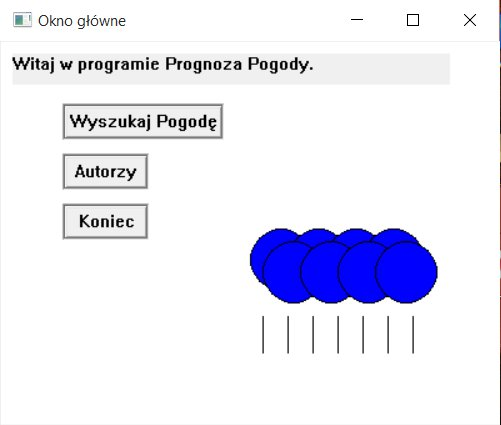
\includegraphics[scale=0.70]{menu.jpg}
\caption{Menu główne.}%
\label{rys:etykieta}
\end{figure} 
Ekran z autorami zawiera elementy typu label z danymi autorów programu (tytuł, imię i nazwisko). Dodatkowo jest przycik zamykający ten ekran.
\begin{figure}[H]
\centering
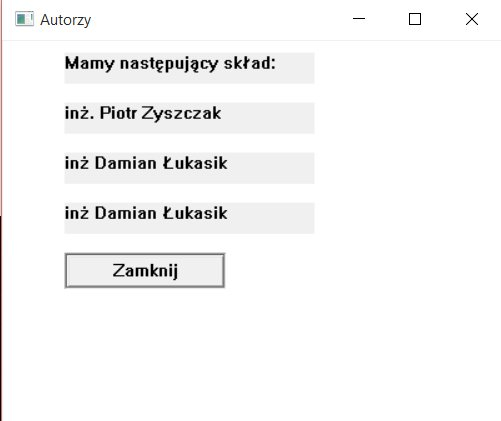
\includegraphics[scale=0.70]{autorzy.jpg}
\caption{Menu główne.}%
\label{rys:etykieta}
\end{figure} 
Nestępne okno zawiera dwie kontrolki z edycją tekstu gdzie można zgodnie z opisem wprowadzić dane potrzebne do zapytania http. Przycisk Sprawdź pogodę wyświetki nam raport z danymi pogodowymi i informacjami o połączeniu. Przycisk testuj bazę łączy z bazą MySQL i  zwraca pobrane z niej rekordy.
\begin{figure}[H]
\centering
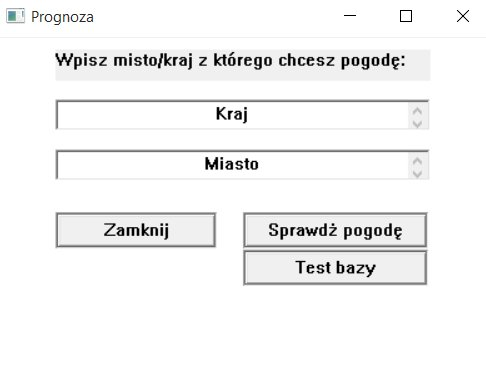
\includegraphics[scale=0.70]{serwis.jpg}
\caption{Menu główne.}%
\label{rys:etykieta}
\end{figure} 
\chapter{Podsumowanie}
Zrealizowano wszystkie założenia projektu:
\begin{itemize}
\item System okienkowyzaimplementowano zgodnie z zaleceniami na zajęciach.
\item Grafika rastrowa zostałą stworzona w oparciu o GDI.
\item Wielowątkowość zaimplementowano w postaci dwóch dodatkowych wątków na połączenie z bazą i pobieranie danych ze strony.
\item Połączono z bazą danych MySQL przy pomocy sterownika ODBC.
\item Zastosowano wątek z obsługą komunikacji sieciowej w technologii z obsługą gniazd bez przejścia z układu I/O na wiadomości systemu windows(R) (winsock.dll)  
\end{itemize}
\end{document}
